\documentclass[13pt,a4paper]{report}
\usepackage[margin=0.6in]{geometry}
\usepackage{fancybox}
\usepackage[utf8]{inputenc}
\usepackage[vietnamese,main=english]{babel}
\usepackage{multicol}
\usepackage{tabularx}
\usepackage{lmodern}
\usepackage{indentfirst}
\usepackage{float}
\usepackage{enumitem}
\usepackage{afterpage}
\usepackage[super]{nth}
\usepackage{titlesec}
\usepackage{bigdelim}
\usepackage[titles]{tocloft}
\usepackage{makecell}
\usepackage{arydshln}
\usepackage{perpage} %the perpage package
\usepackage{graphicx}
\usepackage{caption}
\usepackage{minted}
\usepackage{gensymb}
\usepackage{tikz}
\usepackage{circuitikz}
\usepackage{pgfplots}
\usepackage{cancel}
\usepackage{xurl}
\usepackage[bottom]{footmisc}
\usepackage[font=footnotesize,labelfont={scriptsize}]{subfig}
\usepackage{wrapfig}
\usepackage{latexsym,amssymb,amsmath}
%\usepackage{algpseudocode}
\usepackage{tocvsec2}
\usepackage{fancyref}
\usepackage{bookmark}
\usepackage{hyperref}
\usepackage[nameinlink,noabbrev]{cleveref}

\newcolumntype{Y}{>{\centering\arraybackslash}X}

\PassOptionsToPackage{hyphens}{url}

\makeatletter
\pgfcircdeclarebipole{}{\ctikzvalof{bipoles/vsourceam/height}}{vsourceAM}{\ctikzvalof{bipoles/vsourceam/height}}{\ctikzvalof{bipoles/vsourceam/width}}{%
  \pgfsetlinewidth{\pgfkeysvalueof{/tikz/circuitikz/bipoles/thickness}\pgfstartlinewidth}
   \pgfpathellipse{\pgfpointorigin}{\pgfpoint{0}{\pgf@circ@res@up}}{\pgfpoint{\pgf@circ@res@left}{0}}
   \pgfusepath{draw}
   \pgfscope
       \pgftransformxshift{0.6*\ctikzvalof{bipoles/vsourceam/margin}\pgf@circ@res@left}
       \pgftext[rotate=-\pgf@circ@direction]{$+$}
       \pgfusepath{draw}
   \endpgfscope
   \pgfscope
       \pgftransformxshift{0.6*\ctikzvalof{bipoles/vsourceam/margin}\pgf@circ@res@right}
       \pgftext[rotate=-\pgf@circ@direction]{$-$}
       \pgfusepath{draw}
   \endpgfscope
}
\makeatother

\MakePerPage{footnote} %the perpage package command
\usetikzlibrary{shapes,positioning,arrows,calc,automata}

\newcommand*\justify{%
  \fontdimen2\font=0.4em% interword space
  \fontdimen3\font=0.2em% interword stretch
  \fontdimen4\font=0.1em% interword shrink
  \fontdimen7\font=0.1em% extra space
  \hyphenchar\font=`\-% allowing hyphenation
}
\renewcommand\cftchapafterpnum{\vskip-2pt}
\renewcommand\cftsecafterpnum{\vskip-2pt}

\renewcommand{\theequation}{\arabic{equation}}

% FLOW CHART
\tikzstyle{startstop} = [rectangle, rounded corners, minimum width=3cm, minimum height=1cm,text centered, draw=black, fill=red!30]
\tikzstyle{io} = [trapezium, trapezium left angle=70, trapezium right angle=110, minimum width=3cm, minimum height=1cm, text centered, draw=black, fill=blue!30]
\tikzstyle{process} = [rectangle, minimum width=3cm, minimum height=1cm, text centered, draw=black, fill=orange!30, text width=4cm]
\tikzstyle{decision} = [diamond, aspect=2.5, minimum width=3cm, minimum height=1cm, text centered, draw=black, fill=green!30]
\tikzstyle{arrow} = [thick,->,>=stealth]

% CHAPTER FORMAT
\titleformat{\chapter}%[display]
{\bfseries\fontsize{25}{30}\selectfont\raggedright}% Format and size of title text
{\llap{%
    \rule[-6pt]{6cm}{1.18cm}\rule{6pt}{0pt}}% Black box to the left, lowered 6pt. The end rule is a horisontal space.
  \llap{% Number also to the left, on top of the black box.
    \fontsize{22}{44}\selectfont\color{white}\thechapter\rule{10pt}{0pt}}}{0pt}{}{}

\counterwithin{figure}{section}
\renewcommand{\thefigure}{\arabic{chapter}.\arabic{section}.\alph{figure}}

\renewcommand{\thetable}{\arabic{table}}

\renewcommand\labelitemi{$-$}
  
\titleformat{\section}
  {\LARGE\bfseries}{}{}{}
\renewcommand\thesection{\arabic{section}.}
\renewcommand\thesubsection{\arabic{subsection}}
\makeatletter
\renewcommand*\l@section{\@dottedtocline{1}{1.5cm}{2em}}
\renewcommand\section{\@startsection {section}{1}{-1em}%
  {-3.5ex \@plus -1ex \@minus -.2ex}%
  {2.3ex \@plus.2ex}%
  {\normalfont\Large\bfseries}}
\def\sectionmark#1{%
      \markright {\MakeUppercase{#1}}}
\makeatother

\titleformat{\subsection}
  {\normalfont\bfseries}{\thesubsection.}{0.5em}{}
\renewcommand\cftsubsecaftersnum{.} 
\renewcommand\thesubsection{\alph{subsection}}

\addto{\captionsenglish}{%
  \renewcommand{\bibname}{References}
}

%\addtocontents{toc}{\setcounter{tocdepth}{2}}
%\addtocontents{lof}{\vskip -1.6cm}
%\addtocontents{lot}{\vskip -1.6cm}

    
% TOC settings
\renewcommand\cftchapnumwidth{2.8em}
\renewcommand\cftsecnumwidth{3em}
\renewcommand\cftsecindent{3em}
\renewcommand\cftsubsecindent{5em}
\renewcommand\thechapter{\Roman{chapter}}
    
%\titleformat{\chapter}[display]{\normalfont\huge\bfseries}{}{0pt}{\Huge}
\newcommand{\hsp}{\hspace{20pt}}
%\titleformat{\chapter}[hang]{\Huge\bfseries}{\thechapter\hsp\textcolor{gray75}{|}\hsp}{0pt}{\Huge\bfseries}
\titleformat*{\subsubsection}{\large\bfseries}
%\titlespacing*{\chapter}{0pt}{0pt}{0pt}
    
\newcolumntype{P}[1]{>{\centering\arraybackslash}p{#1}}
\newcolumntype{C}{>{\centering\arraybackslash}p{4em}}
    
\setlist[itemize]{noitemsep, topsep=0pt}
%\AtBeginEnvironment{multicols}{\RaggedRight}

\titlespacing*{\chapter}{0pt}{0pt}{20pt}

\newcommand\Chapter[2]{\chapter
  [#1\text{: }\hfil\hbox{}\protect\linebreak{\itshape#2}]%
  {#1\\[-0.75ex]\Large#2}%
  \markboth{\MakeUppercase{\chaptername\ \thechapter.\ #1}}{}%
}


\def\doubleoverline#1{\overline{\overline{#1}}}

\captionsetup[subfloat]{labelformat=empty}

\begin{document}
%Trang bìa 1
\fontsize{13pt}{18pt}\selectfont
\begin{titlepage}
\thispagestyle{empty}
\thisfancypage{%đóng khung trang này
\setlength{\fboxsep}{0pt}% 8pt là độ dày của đường viền
\fbox}{} % phần nội dung sau là tương tự như đã làm
\

\begin{center}
\begin{large}
HO CHI MINH CITY UNIVERSITY OF TECHNOLOGY $-$ VNU HCMC
\end{large} \\
\begin{large}
OFFICE FOR INTERNATIONAL STUDY PROGRAM
\end{large} \\
\begin{large}
FACULTY OF ELECTRICAL AND ELECTRONIC ENGINEERING
\end{large} \\
\textbf{--------------------  *  --------------------}\\[4cm]

\includegraphics[scale=0.1]{logobk.png}\\[1cm]
{\fontsize{20pt}{1}\selectfont DIGITAL SYSTEMS (LAB)}\\
{\fontsize{20pt}{1}\selectfont EXPERIMENTAL REPORT (Lab 5)}\\[2.5cm]
\end{center}

\begin{otherlanguage}{vietnamese}
\begin{tabbing}
	\hspace{3.5cm}Lecturer  \ \ \ \ \=: \textbf{\parbox[t]{9cm}{Mr. Nguyễn Tuấn Hùng}}\\
	\hspace{3.5cm}Subject \>: \textbf{\parbox[t]{12cm}{Digital Systems}}\\
	\hspace{3.5cm}Class \>: \textbf{\parbox[t]{9cm}{TT06}}\\
	\hspace{3.5cm}Name \>: \textbf{\parbox[t]{9cm}{
		Lương Triển Thắng}}\\
	\hspace{3.5cm}Student ID \>: \textbf{\parbox[t]{9cm}{
		2051194}}\\[40pt]
\end{tabbing}
\end{otherlanguage}

\vspace{2.25cm}
\begin{center}
{\fontsize{13pt}{1}\selectfont Ho Chi Minh City, \nth{14} June, 2022}
\end{center}
\end{titlepage}

\tableofcontents

\setminted{fontsize=\normalsize}

\setcounter{chapter}{4}

\Chapter{Laboratory 5}{A simple processor}

\section{Design and implement a simple processor}
\subsection{Code}

\subsubsection{DFF.vhd}
\begin{minted}{vhdl}
LIBRARY ieee;
USE ieee.std_logic_1164.ALL;
ENTITY DFFn IS
	PORT (
		D, clk, rst, en : IN STD_LOGIC;
		Q : OUT STD_LOGIC);
END DFFn;
ARCHITECTURE Behavior OF DFFn IS
BEGIN
	PROCESS (rst, clk, en)
	BEGIN
		IF rst = '1' THEN
			Q <= '0';
		ELSIF rising_edge(clk) AND en = '1' THEN
			Q <= D;
		END IF;
	END PROCESS;
END Behavior;
\end{minted}

\subsubsection{myReg.vhd}
\begin{minted}{vhdl}
LIBRARY ieee;
USE ieee.std_logic_1164.ALL;
USE ieee.numeric_std.ALL;

ENTITY myReg IS
	PORT (
		clk, rst, en : IN STD_LOGIC;
		D : IN STD_LOGIC_VECTOR(8 DOWNTO 0);
		Q : OUT STD_LOGIC_VECTOR(8 DOWNTO 0)
	);
END myReg;

ARCHITECTURE arch OF myReg IS
	COMPONENT DFFn IS
		PORT (
			D, clk, rst, en : IN STD_LOGIC;
			Q : OUT STD_LOGIC);
	END COMPONENT;
BEGIN
	gen : FOR i IN 8 DOWNTO 0 GENERATE
		DFFs : DFFn PORT MAP(D(i), clk, rst, en, Q(i));
	END GENERATE;
END ARCHITECTURE;
\end{minted}

\subsubsection{RegMUX.vhd}
\begin{minted}{vhdl}
LIBRARY ieee;
USE ieee.std_logic_1164.ALL;
USE ieee.numeric_std.ALL;

ENTITY regMUX IS
	PORT (
		SIGNAL R0, R1, R2, R3, R4, R5, R6, R7 : IN STD_LOGIC_VECTOR(8 DOWNTO 0);
		SIGNAL g, DIN : IN STD_LOGIC_VECTOR(8 DOWNTO 0);
		SIGNAL sel : IN INTEGER RANGE 0 TO 10;
		SIGNAL MUXout : OUT STD_LOGIC_VECTOR(8 DOWNTO 0)
	);
END regMUX;

ARCHITECTURE arch OF regMUX IS
BEGIN
	WITH sel SELECT
		MUXout <=
		R0 WHEN 0,
		R1 WHEN 1,
		R2 WHEN 2,
		R3 WHEN 3,
		R4 WHEN 4,
		R5 WHEN 5,
		R6 WHEN 6,
		R7 WHEN 7,
		g WHEN 8,
		DIN WHEN 9,
		"000000000" WHEN 10;
END ARCHITECTURE;
\end{minted}

\subsubsection{AddSub.vhd}
\begin{minted}{vhdl}
LIBRARY ieee;
USE ieee.std_logic_1164.ALL;
USE ieee.numeric_std.ALL;

ENTITY AddSub IS
    PORT (
        SIGNAL A, B : IN STD_LOGIC_VECTOR(8 DOWNTO 0);
        SIGNAL sel : IN STD_LOGIC;
        SIGNAL C : OUT STD_LOGIC_VECTOR(8 DOWNTO 0)
    );
END AddSub;

ARCHITECTURE arch OF AddSub IS
BEGIN
C <= STD_LOGIC_VECTOR(UNSIGNED(A) + UNSIGNED(B)) WHEN sel = '0' ELSE
        STD_LOGIC_VECTOR(UNSIGNED(A) - UNSIGNED(B));
END ARCHITECTURE;
\end{minted}

\subsubsection{ctrlunitFSM.vhd}
\begin{minted}{vhdl}
LIBRARY ieee;
USE ieee.std_logic_1164.ALL;
USE ieee.numeric_std.ALL;

ENTITY ctrlunitFSM IS
	PORT (
		SIGNAL rin : OUT STD_LOGIC_VECTOR(0 TO 7);
		SIGNAL ain, gin, IRin, addsub : OUT STD_LOGIC;
		SIGNAL IR : IN STD_LOGIC_VECTOR(8 DOWNTO 0);
		SIGNAL outsel : OUT INTEGER RANGE 0 TO 10;
		SIGNAL run, rst, clk : IN STD_LOGIC;
		SIGNAL done : BUFFER STD_LOGIC
	);
END ctrlunitFSM;

ARCHITECTURE arch OF ctrlunitFSM IS
	TYPE State_type IS (T0, T1, T2, T3);
	SIGNAL Tstep_Q, Tstep_D : State_type;

	SIGNAL opcode : STD_LOGIC_VECTOR(2 DOWNTO 0);
	SIGNAL RX, RY : NATURAL RANGE 0 TO 7;
BEGIN
	opcode <= IR(8 DOWNTO 6);
	RX <= TO_INTEGER(UNSIGNED(IR(5 DOWNTO 3)));
	RY <= TO_INTEGER(UNSIGNED(IR(2 DOWNTO 0)));
	statetable :
	PROCESS (Tstep_D, run)
	BEGIN
		CASE Tstep_D IS
			WHEN T0 =>
				IF run = '0' THEN
					Tstep_Q <= T0;
				ELSE
					Tstep_Q <= T1;
				END IF;
				-- data IS loaded into IR IN this TIME step
			WHEN T1 =>
				IF done = '1' THEN
					TStep_Q <= T0;
				ELSE
					Tstep_Q <= T2;
				END IF;
			WHEN T2 =>
				Tstep_Q <= T3;
			WHEN T3 =>
				IF done = '1' THEN
					TStep_Q <= T0;
				ELSE
					-- ERROR
				END IF;
			WHEN OTHERS => NULL;
		END CASE;
	END PROCESS;

	controlsignals :
	PROCESS (Tstep_D, IR, opcode, RX, RY)
	BEGIN
		rin <= (OTHERS => '0');
		ain <= '0';
		gin <= '0';
		outsel <= 10;
		addsub <= '0';
		CASE Tstep_D IS
			WHEN T0 => -- store DIN IN IR as long as Tstep_Q = 0
				IRin <= '1';
				done <= '0';
				outsel <= 9;
			WHEN T1 =>
				CASE opcode IS
					WHEN "000" =>
						outsel <= RY;
						done <= '1';
						rin(RX) <= '1';
					WHEN "001" =>
						outsel <= 9;
						done <= '1';
						rin(RX) <= '1';
					WHEN "010" | "011" =>
						outsel <= RX;
						ain <= '1';
					WHEN OTHERS => NULL;
				END CASE;
			WHEN T2 =>
				CASE opcode IS
					WHEN "010" =>
						outsel <= RY;
						gin <= '1';
					WHEN "011" =>
						outsel <= RY;
						gin <= '1';
						addsub <= '1';
					WHEN OTHERS => NULL;
				END CASE;
			WHEN T3 =>
				CASE opcode IS
					WHEN "010" | "011" =>
						outsel <= 8;
						rin(RX) <= '1';
						done <= '1';
					WHEN OTHERS => NULL;
				END CASE;
			WHEN OTHERS => NULL;
		END CASE;
	END PROCESS;
	flipflops : PROCESS (clk, rst, Tstep_Q)
	BEGIN
		IF rst = '1' THEN
			Tstep_D <= T0;
		ELSIF rising_edge(clk) THEN
			Tstep_D <= Tstep_Q;
		END IF;
	END PROCESS;
END ARCHITECTURE;
\end{minted}

\subsubsection{Exc1.vhd}
\begin{minted}{vhdl}
LIBRARY ieee;
USE ieee.std_logic_1164.ALL;
USE ieee.numeric_std.ALL;

ENTITY Exc1 IS
	PORT (
		R0out, R1out, Aout, Gout, IRout : OUT STD_LOGIC_VECTOR(8 DOWNTO 0);
		DIN : IN STD_LOGIC_VECTOR(8 DOWNTO 0);
		rstN, clk, run : IN STD_LOGIC;
		done : BUFFER STD_LOGIC;
		BusWires : BUFFER STD_LOGIC_VECTOR(8 DOWNTO 0)
	);
END Exc1;

ARCHITECTURE Behavior OF Exc1 IS
	-- MISC
	SIGNAL addOrSub : STD_LOGIC;

	-- REGISTERS, A, G, IR
	SIGNAL regin : STD_LOGIC_VECTOR(0 TO 7);
	SIGNAL A, G, Gt : STD_LOGIC_VECTOR(8 DOWNTO 0);
	SIGNAL ain, gin, IRin, rst : STD_LOGIC;
	SIGNAL R0, R1, R2, R3, R4, R5, R6, R7, IR : STD_LOGIC_VECTOR(8 DOWNTO 0);
	SIGNAL sel : INTEGER RANGE 0 TO 10;

	COMPONENT myReg IS
		PORT (
			clk, rst, en : IN STD_LOGIC;
			D : IN STD_LOGIC_VECTOR(8 DOWNTO 0);
			Q : OUT STD_LOGIC_VECTOR(8 DOWNTO 0)
		);
	END COMPONENT;

	COMPONENT AddSub IS
		PORT (
			SIGNAL A, B : IN STD_LOGIC_VECTOR(8 DOWNTO 0);
			SIGNAL sel : IN STD_LOGIC;
			SIGNAL C : OUT STD_LOGIC_VECTOR(8 DOWNTO 0)
		);
	END COMPONENT;

BEGIN
	R0out <= R0;
	R1out <= R1;
	Aout <= A;
	Gout <= G;
	IRout <= IR;

	rst <= NOT(rstN);
	-- ADDSUB
	as : AddSub PORT MAP(A, BusWires, addOrSub, Gt);

	-- REGS
	reg0 : myReg PORT MAP(clk, rst, regin(0), BusWires, R0);
	reg1 : myReg PORT MAP(clk, rst, regin(1), BusWires, R1);
	reg2 : myReg PORT MAP(clk, rst, regin(2), BusWires, R2);
	reg3 : myReg PORT MAP(clk, rst, regin(3), BusWires, R3);
	reg4 : myReg PORT MAP(clk, rst, regin(4), BusWires, R4);
	reg5 : myReg PORT MAP(clk, rst, regin(5), BusWires, R5);
	reg6 : myReg PORT MAP(clk, rst, regin(6), BusWires, R6);
	reg7 : myReg PORT MAP(clk, rst, regin(7), BusWires, R7);
	Areg : myReg PORT MAP(clk, rst, ain, BusWires, A);
	Greg : myReg PORT MAP(clk, rst, Gin, Gt, G);
	IRreg : myReg PORT MAP(clk, rst, IRin, DIN, IR);

	-- MUX
	regMUX0 : ENTITY work.RegMUX PORT MAP(R0, R1, R2, R3, R4, R5, R6, R7, G, DIN, sel, BusWires);

	-- FSM
	ControlUnit : ENTITY work.ctrlUnitFSM PORT MAP(
		regin, ain, gin, IRin, addorsub, IR, sel, run, rst, clk, done
	);

END ARCHITECTURE;
\end{minted}

\subsection{Waveform}
\begin{figure}[H]
\centering
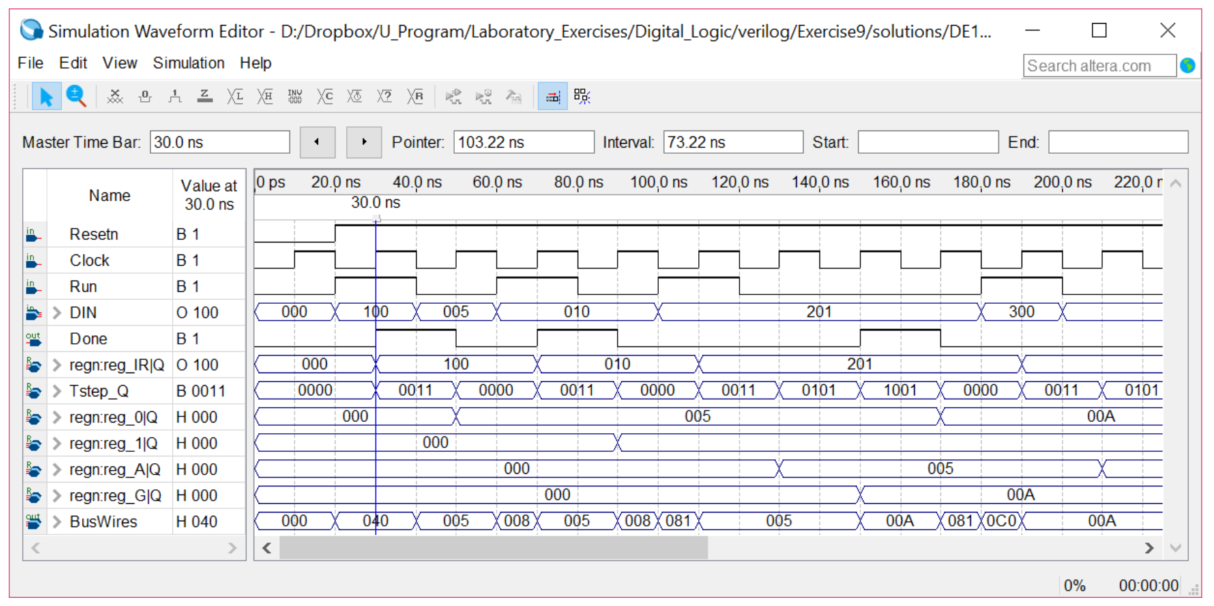
\includegraphics[scale=0.4]{images/Exc1_waveform_ref.png}
\caption*{Reference waveform}
\end{figure}

\begin{figure}[H]
\centering
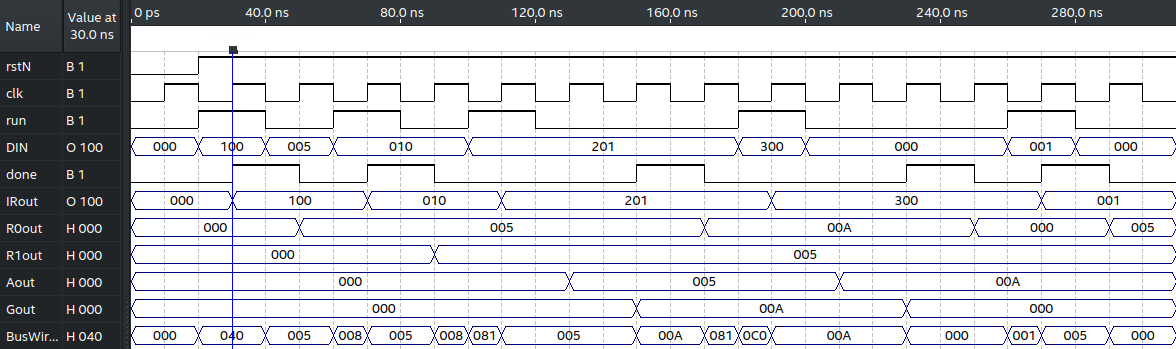
\includegraphics[scale=0.55]{images/Exc1_waveform.png}
\caption*{Simulation result}
\end{figure}

\newpage
\subsection{Result of RTL viewer}
\begin{figure}[H]
\centering
\subfloat[][D flip-flop]{
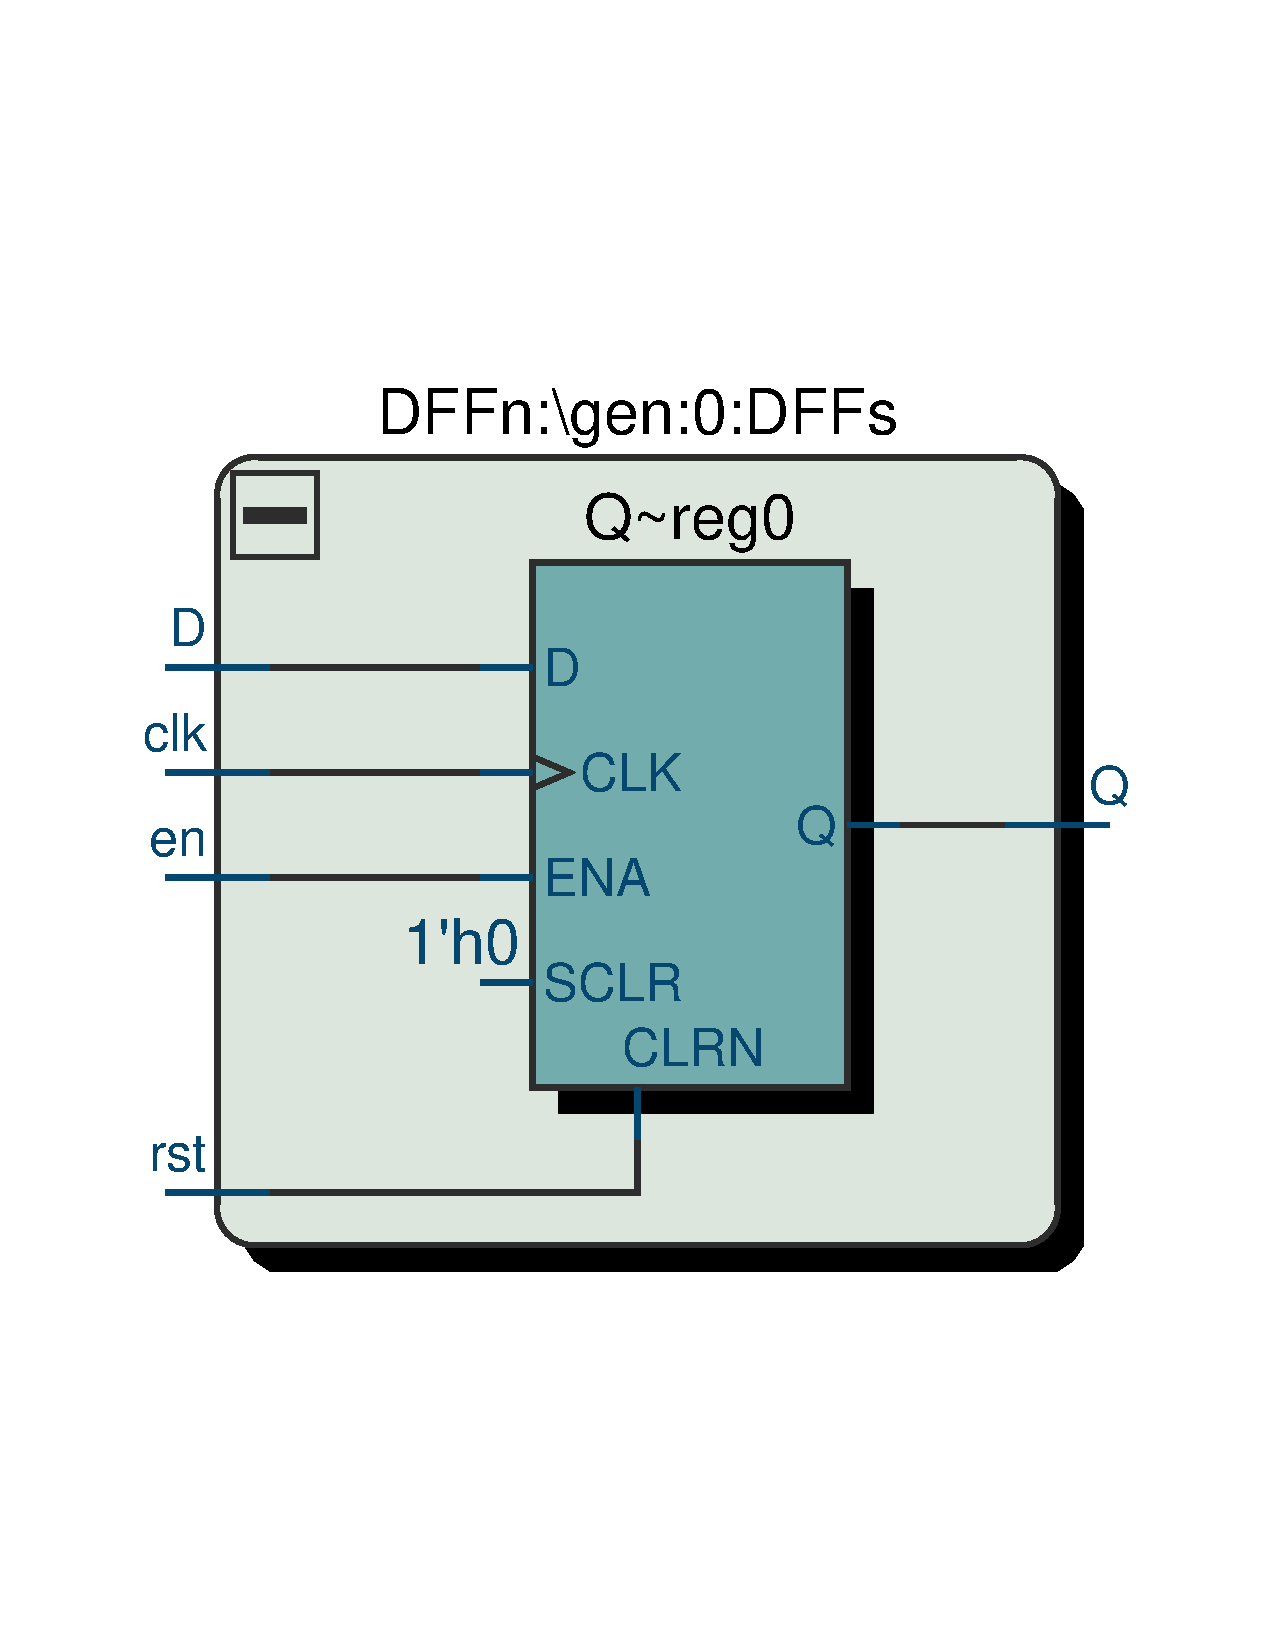
\includegraphics[scale=0.25, clip, trim={0cm 6.5cm 0cm 7.6cm}]{images/Exc1_DFF_RTL.pdf}
}
\subfloat[][Add-Sub]{
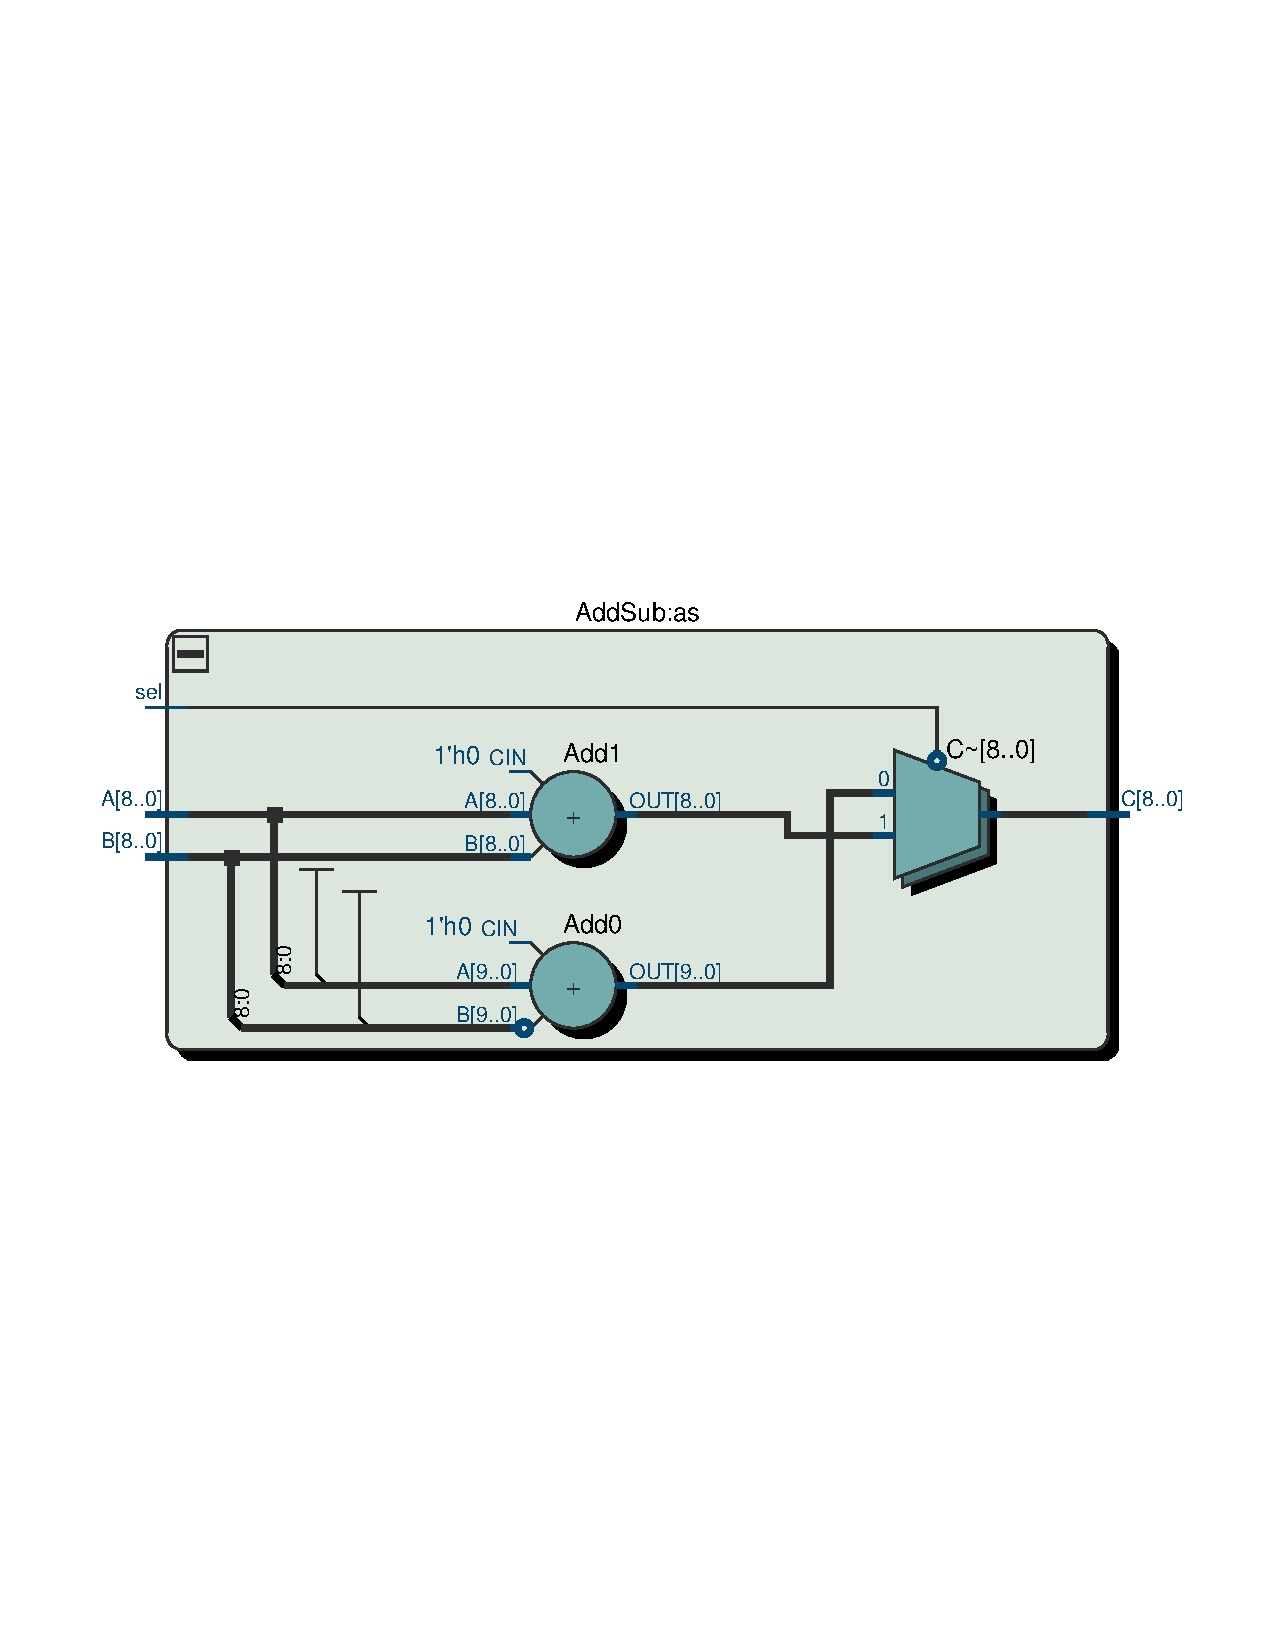
\includegraphics[scale=0.5, clip, trim={0cm 10cm 0cm 10.6cm}]{images/Exc1_AddSub_RTL.pdf}
}
\end{figure}

\begin{figure}[H]
\centering
\subfloat[][Registers MUX]{
\includegraphics[scale=0.6, clip, trim={2cm 1cm 2cm 1.55cm}]{images/Exc1_RegMUX_RTL.pdf}
}
\subfloat[][9-bit register]{
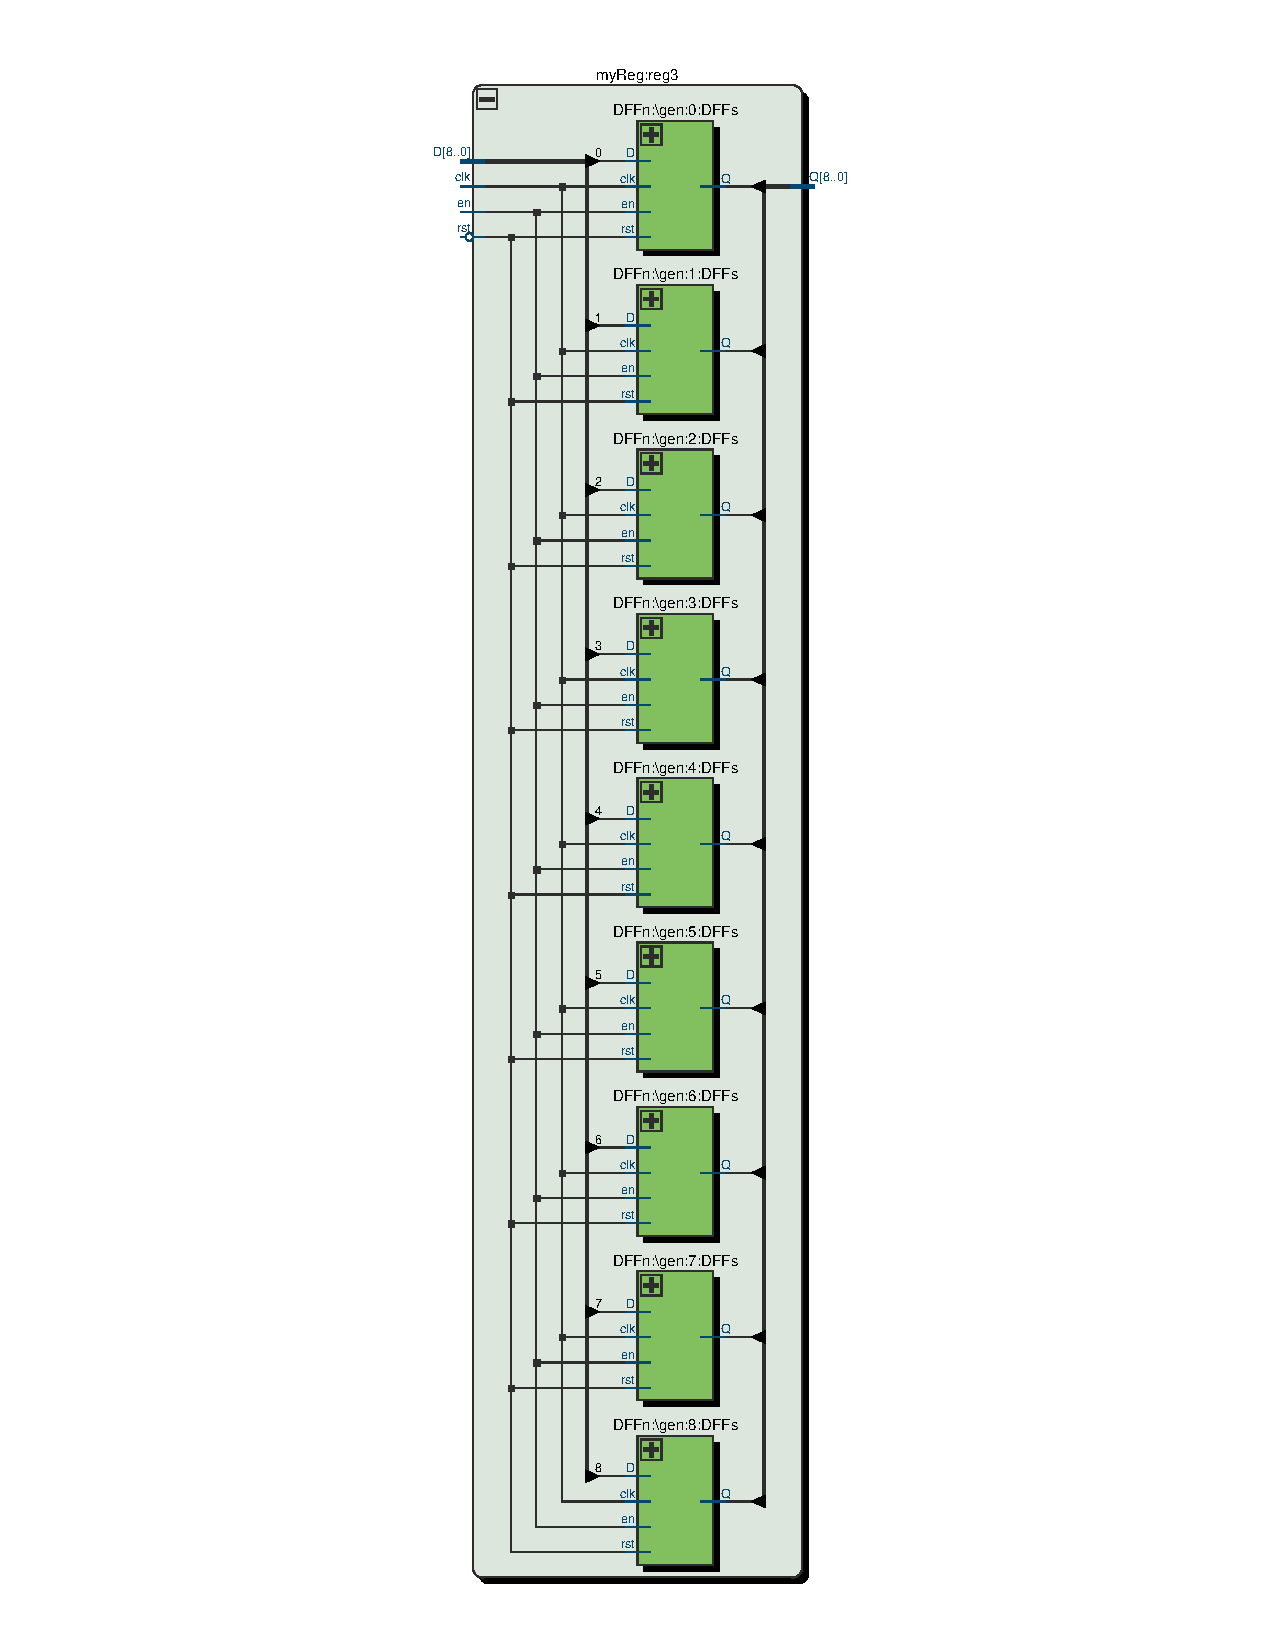
\includegraphics[scale=0.6, clip, trim={4cm 1cm 4cm 1.45cm}]{images/Exc1_myReg_RTL.pdf}
}
\end{figure}

\begin{figure}[H]
\centering
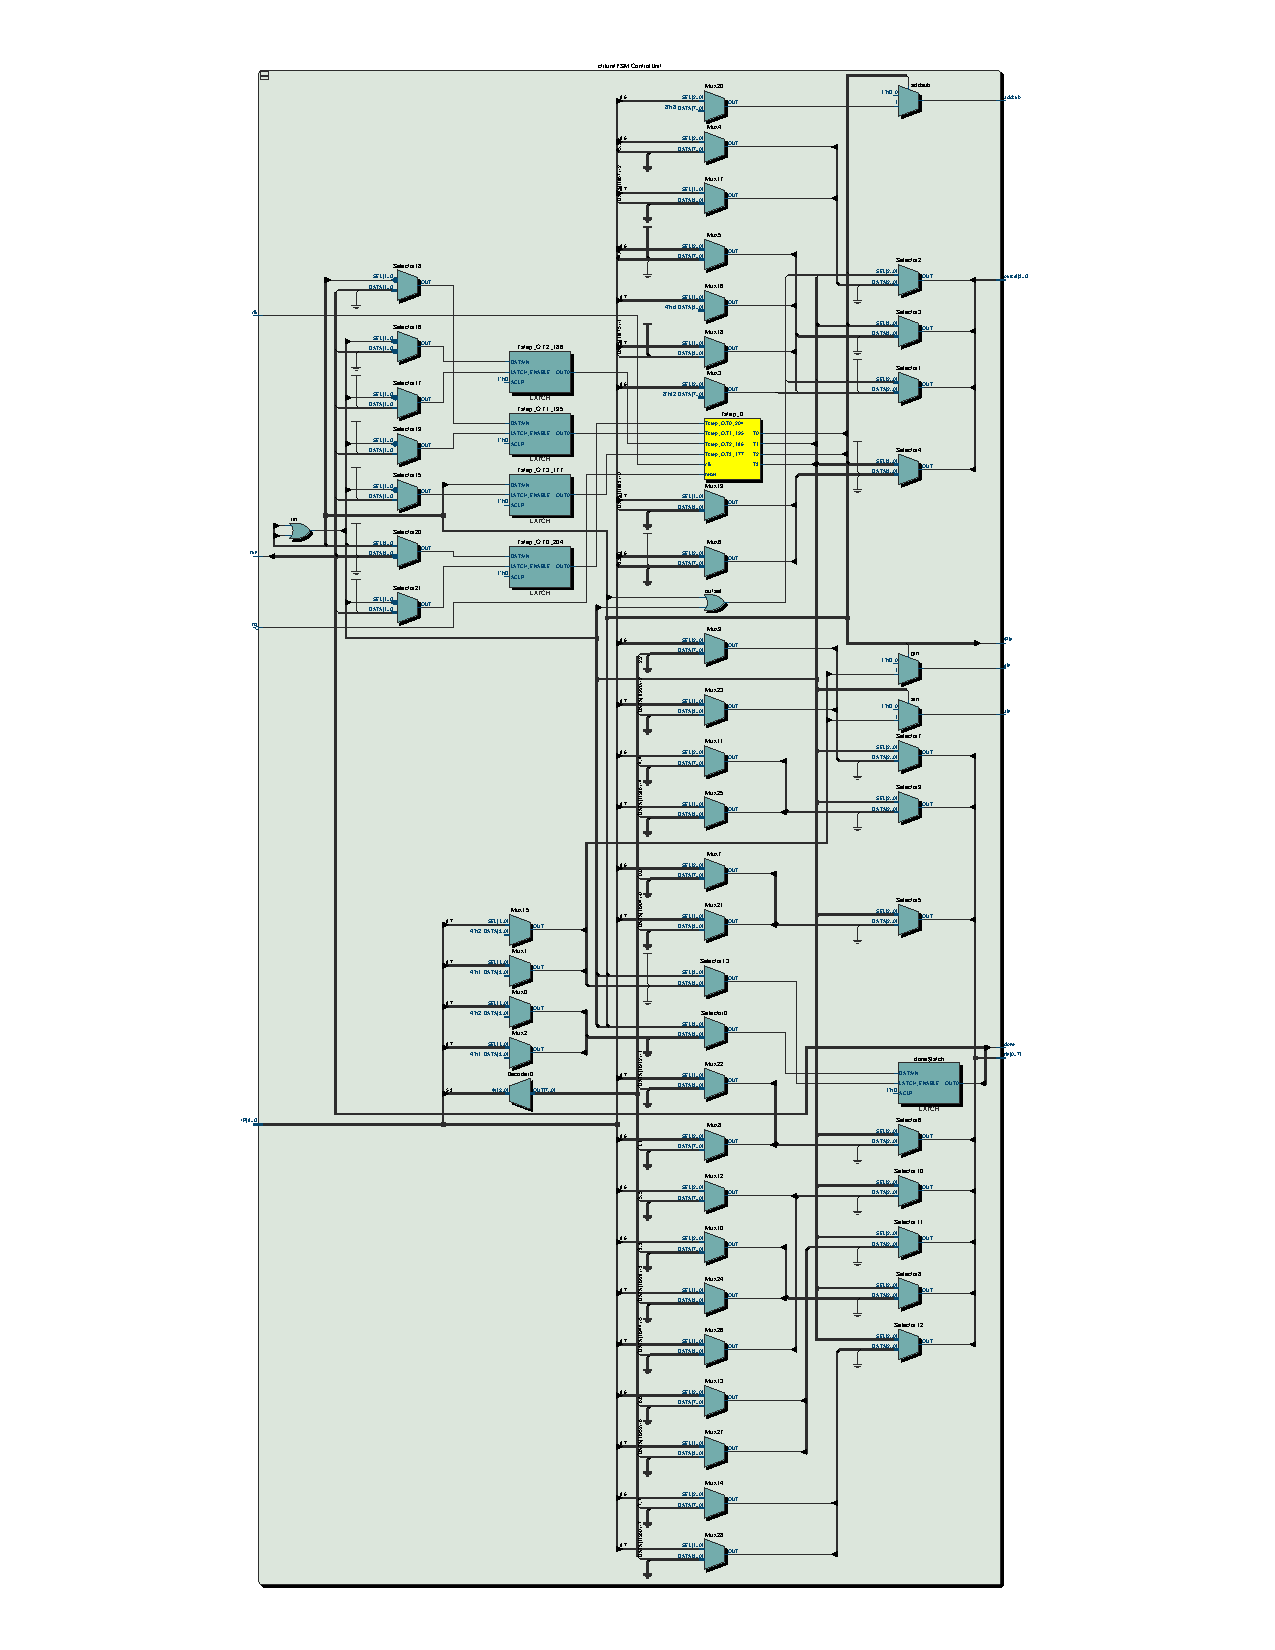
\includegraphics[scale=1, clip, trim={2cm 1cm 2cm 1.2cm}]{images/Exc1_ctrlUnit_RTL.pdf}
\caption*{Control Unit (zoom in for better viewing)}
\end{figure}

\begin{figure}[H]
\centering
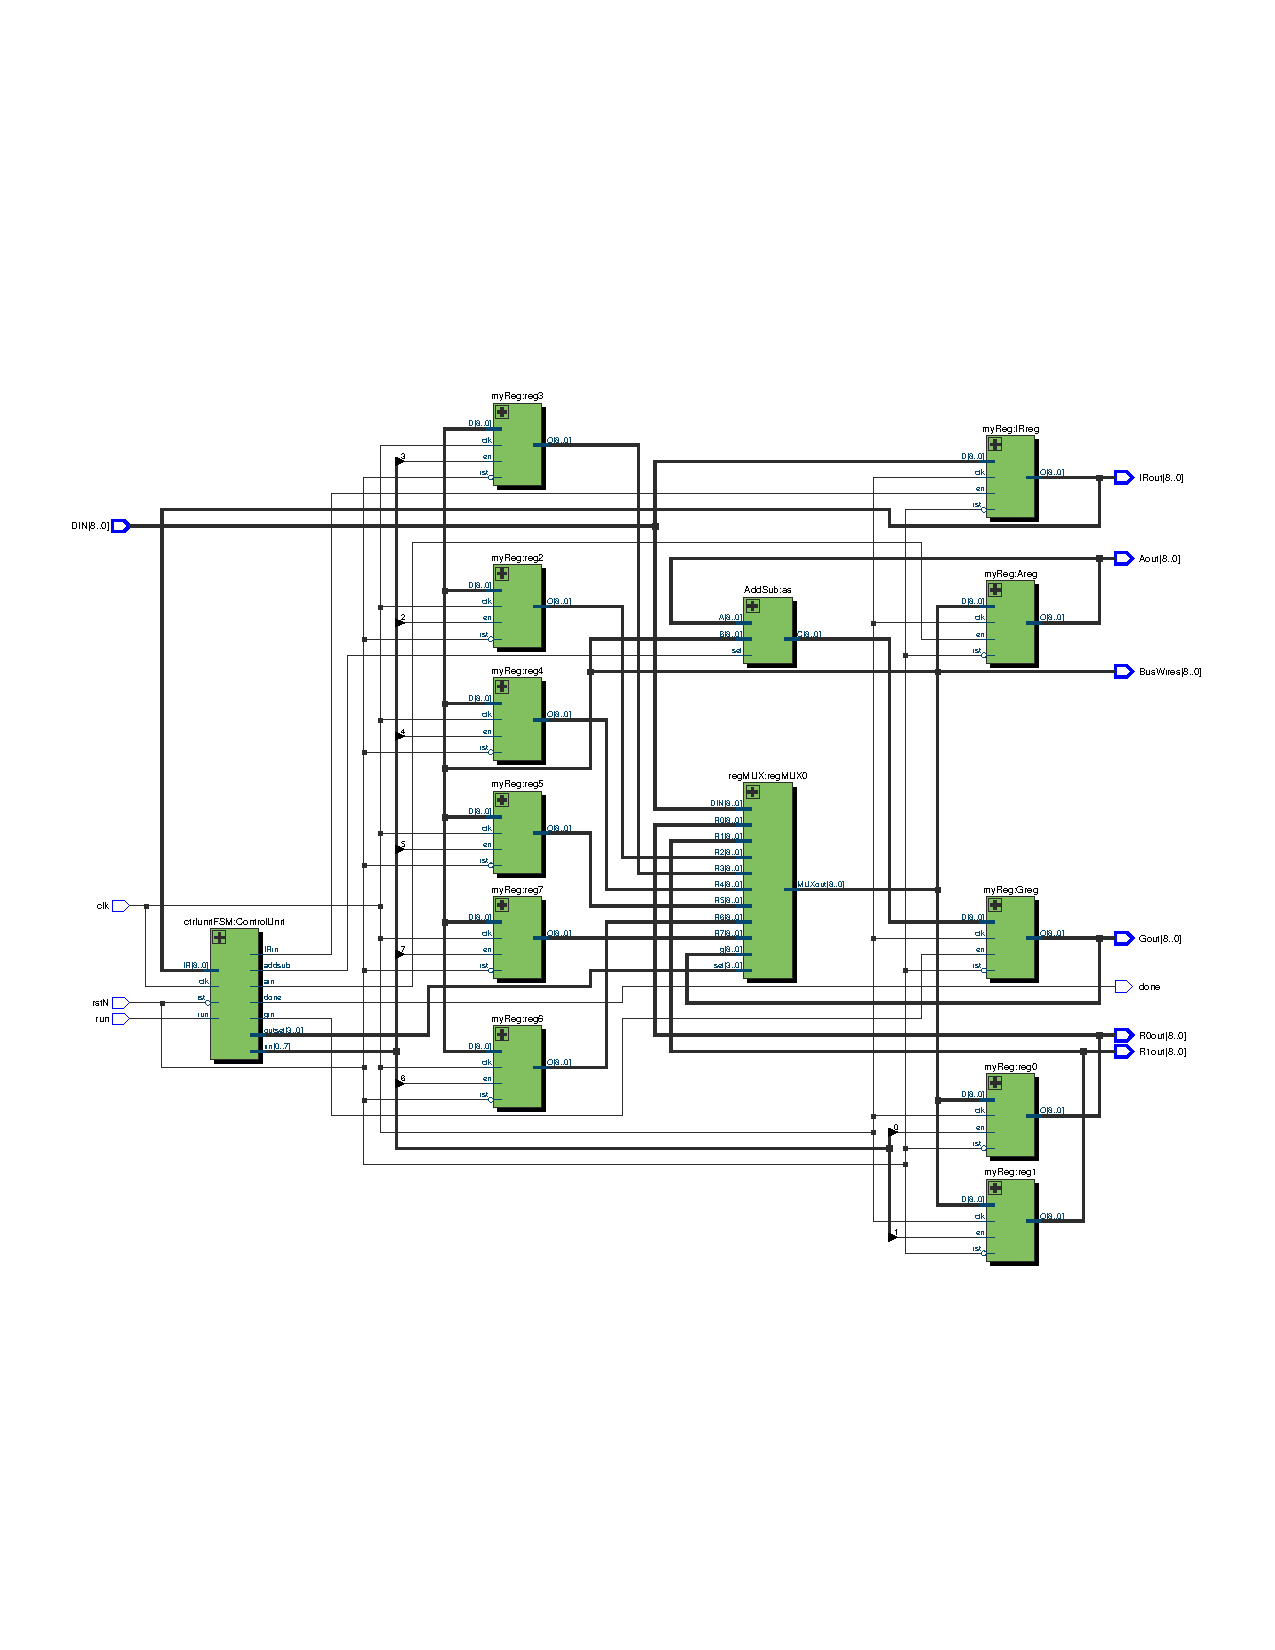
\includegraphics[scale=0.85, clip, trim={0cm 6.5cm 0cm 6.5cm}]{images/Exc1_RTL.pdf}
\caption*{Top level (zoom in for better viewing)}
\end{figure}

\newpage
\section{Design and implement a simple processor with memory}
This exercise is just an extenstion of the previous, so I just propose the additional parts.

I will change the circuit, so that `\texttt{run}' will be not required to set manually in waveform, but in the ROM itself instead. A ROM data now contains 10 bits with MSB is `\texttt{run}'. See the code section for the ROM and waveform to learn more.

A better version of this processor will be introduced in the report of Lab6.
 
\subsection{Code}

\subsubsection{myROM.vhd}
\begin{minted}{vhdl}
LIBRARY ieee;
USE ieee.std_logic_1164.ALL;
USE ieee.numeric_std.ALL;

ENTITY myROM IS
	GENERIC (
		addr_width : INTEGER := 32; -- store 32 elements
		addr_bits : INTEGER := 5; -- required bits to store 32 elements
		data_width : INTEGER := 10 -- each element has 10-bits
	);
	PORT (
		addr : IN STD_LOGIC_VECTOR(addr_bits - 1 DOWNTO 0);
		data, nextData : OUT STD_LOGIC_VECTOR(data_width - 1 DOWNTO 0)
	);
END myROM;

ARCHITECTURE arch OF myROM IS
	TYPE rom_type IS ARRAY (0 TO addr_width - 1) OF STD_LOGIC_VECTOR(data_width - 1 DOWNTO 0);
	SIGNAL user_ROM : rom_type;
	SIGNAL address : INTEGER RANGE 0 TO addr_width - 1;

	ATTRIBUTE ram_init_file : STRING;
	ATTRIBUTE ram_init_file OF user_ROM : SIGNAL IS "rom_data.mif";

BEGIN
	address <= to_integer(unsigned(addr));
	data <= user_ROM (address);
	nextData <= user_ROM (address + 1);
END arch;
\end{minted}

\subsubsection{rom\_data.mif}
\begin{minted}{vhdl}
WIDTH=10;
DEPTH=32;

ADDRESS_RADIX=UNS;
DATA_RADIX=BIN;

CONTENT BEGIN
	[0..31]  :   0000000000;
	0 : 0000000000;
	1 : 1001000000;
	2 : 0000000101;
	3 : 1000001000;
	4 : 1010000001;
	5 : 1011000000;
	6 : 1000000001;
END;
\end{minted}

\subsubsection{Exc2.vhd}
\begin{minted}{vhdl}
LIBRARY ieee;
USE ieee.std_logic_1164.ALL;
USE ieee.numeric_std.ALL;

ENTITY Exc2 IS
  PORT (
    clk, rstN : IN STD_LOGIC;
    run, done : BUFFER STD_LOGIC;
    addrout : OUT STD_LOGIC_VECTOR(4 DOWNTO 0);
    dataOut : OUT STD_LOGIC_VECTOR(9 DOWNTO 0);
    R0out, R1out, Aout, Gout, IRout : OUT STD_LOGIC_VECTOR(8 DOWNTO 0);
    busWires : OUT STD_LOGIC_VECTOR(8 DOWNTO 0)
  );
END Exc2;

ARCHITECTURE arch OF Exc2 IS
  -- signal to store received data
  SIGNAL data, nextData : STD_LOGIC_VECTOR (9 DOWNTO 0);
  SIGNAL IR : STD_LOGIC_VECTOR(8 DOWNTO 0);
  SIGNAL addr : STD_LOGIC_VECTOR(4 DOWNTO 0) := "00000";
  SIGNAL mclk, isIR : STD_LOGIC;

  TYPE states IS (T0, T1, T2);
  SIGNAL state : states;

  COMPONENT Exc1 IS
    PORT (
      R0out, R1out, Aout, Gout, IRout : OUT STD_LOGIC_VECTOR(8 DOWNTO 0);
      DIN : IN STD_LOGIC_VECTOR(8 DOWNTO 0);
      rstN, clk, run : IN STD_LOGIC;
      done : BUFFER STD_LOGIC;
      BusWires : BUFFER STD_LOGIC_VECTOR(8 DOWNTO 0)
    );
  END COMPONENT;
BEGIN
  user_ROM : ENTITY work.myROM PORT MAP (addr, data, nextData);

  processor : Exc1 PORT MAP(R0out, R1out, Aout, Gout, IRout, IR, rstN, clk, run, done, busWires);

  run <= data(9);
  IR <= data(8 DOWNTO 0);

  addrout <= addr;
  dataOut <= data;

  PROCESS (clk, rstN, done)
  BEGIN
    IF rstN = '0' THEN
      state <= T0;
      addr <= "00000";
    ELSIF falling_edge(clk) THEN
      CASE state IS
        WHEN T0 =>
          addr <= STD_LOGIC_VECTOR(UNSIGNED(addr) + 1);
          state <= T1;
        WHEN T1 =>
          IF done = '1' THEN
            IF nextData(9) = '0' THEN
              addr <= STD_LOGIC_VECTOR(UNSIGNED(addr) + 1);
            END IF;
            state <= T0;
          ELSE
            state <= T1;
          END IF;
        WHEN T2 => NULL;
      END CASE;
    END IF;
  END PROCESS;
END arch;
\end{minted}

\subsection{Waveform}
\begin{figure}[H]
\centering
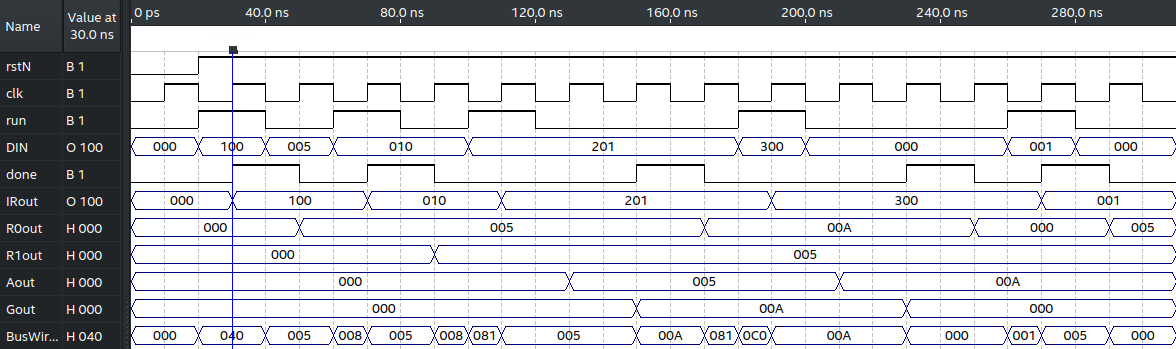
\includegraphics[scale=0.55]{images/Exc1_waveform.png}
\caption*{Simulation result of Exc1}
\end{figure}

\begin{figure}[H]
\centering
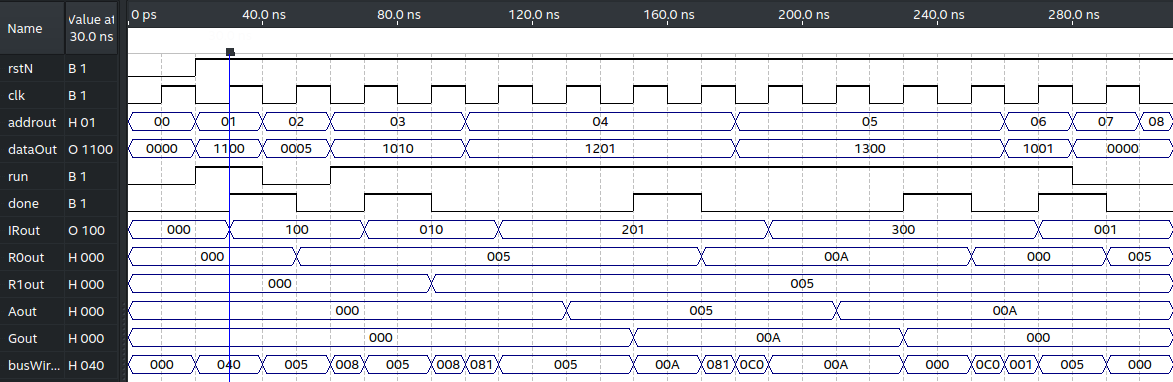
\includegraphics[scale=0.55]{images/Exc2_waveform.png}
\caption*{Simulation result}
\end{figure}

\subsection{Result of RTL viewer}
\begin{figure}[H]
\centering
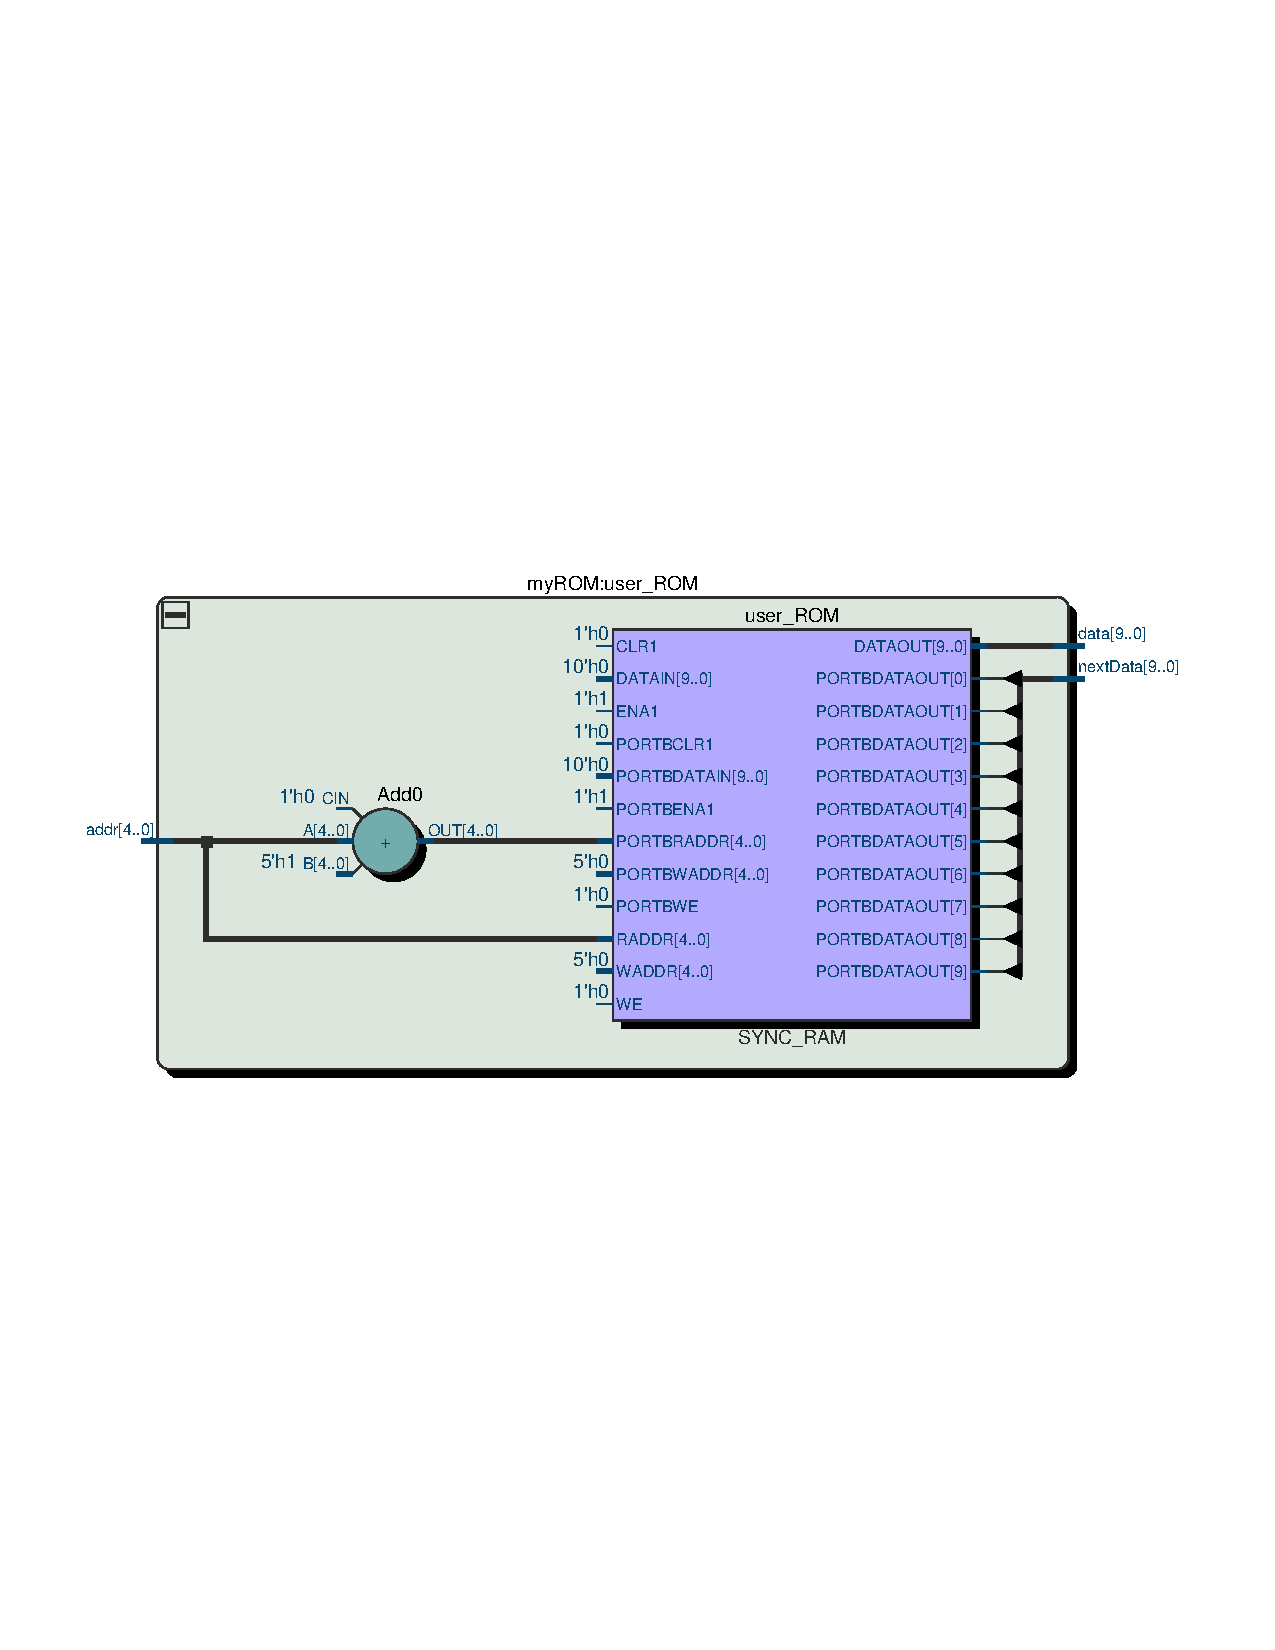
\includegraphics[scale=0.8, clip, trim={0cm 9.5cm 0cm 10.1cm}]{images/Exc2_myROM_RTL.pdf}
\caption*{Read-only memory (ROM)}
\end{figure}

\begin{figure}[H]
\centering
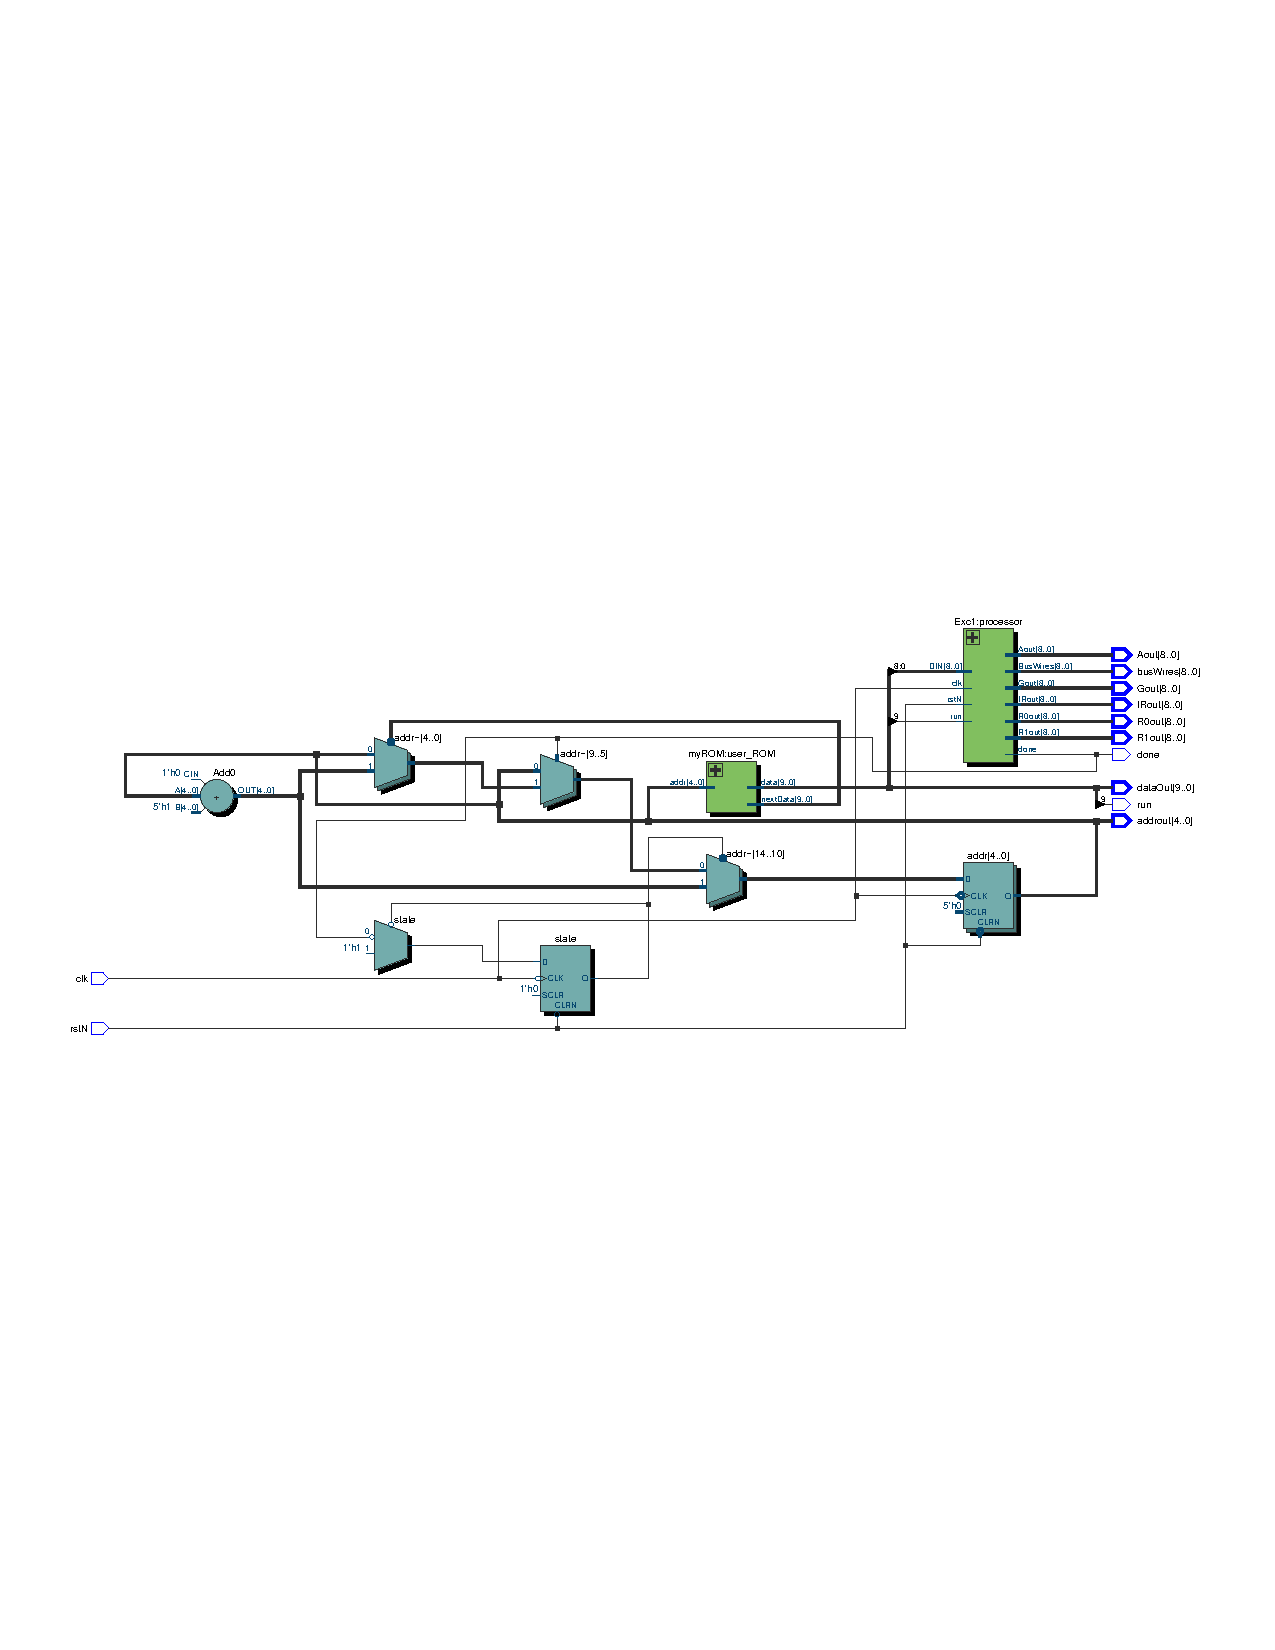
\includegraphics[scale=0.9, clip, trim={1cm 10cm 1cm 10cm}]{images/Exc2_RTL.pdf}
\caption*{Top level (zoom in for better viewing)}
\end{figure}

\end{document}